% The simple model figure (fig:architecture), in words, no symbols. Greys, words of the text (review 2026-11-24). Left, one
% agent's network. Right, every agent running it, conflict resolution and the
% warehouse. The full network with its layers is architecture_detail.tex
% (Appendix C). Adapted from Figure 3 of van Knippenberg et al. (2021).
% Build:  latexmk -pdf architecture.tex, then copy architecture.pdf to Images/.
\documentclass[border=2pt]{standalone}
\usepackage{lmodern}
\usepackage[T1]{fontenc}
\usepackage{amsmath,amssymb}
\usepackage{tikz}
\usetikzlibrary{positioning,fit,backgrounds,arrows.meta,calc,decorations.pathreplacing}

% Greys only, as Figure 12 (methodloop.tex).
\definecolor{shareF}{HTML}{F3F5F7}
\definecolor{agentF}{HTML}{DDE1E6}
\definecolor{ink}{HTML}{43505C}
\definecolor{muted}{HTML}{5A6673}

\tikzset{
  layer/.style={draw=ink, line width=0.8pt, rounded corners=3pt, align=center,
                fill=shareF, text width=5.4cm, minimum height=0.95cm,
                inner sep=4pt, font=\small},
  head/.style={draw=ink, line width=0.8pt, rounded corners=3pt, align=center,
               fill=shareF, text width=2.55cm, minimum height=1.05cm,
               inner sep=3pt, font=\small},
  agent/.style={draw=ink, line width=0.8pt, rounded corners=3pt, fill=agentF,
                minimum width=1.7cm, minimum height=0.8cm, font=\small},
  sys/.style={draw=ink, line width=0.8pt, rounded corners=3pt, align=center,
              minimum height=0.9cm, inner sep=4pt, font=\small},
  flow/.style={-{Stealth[length=2.4mm]}, line width=0.9pt, draw=ink},
  lbl/.style={font=\footnotesize, text=ink, align=center},
}

\begin{document}
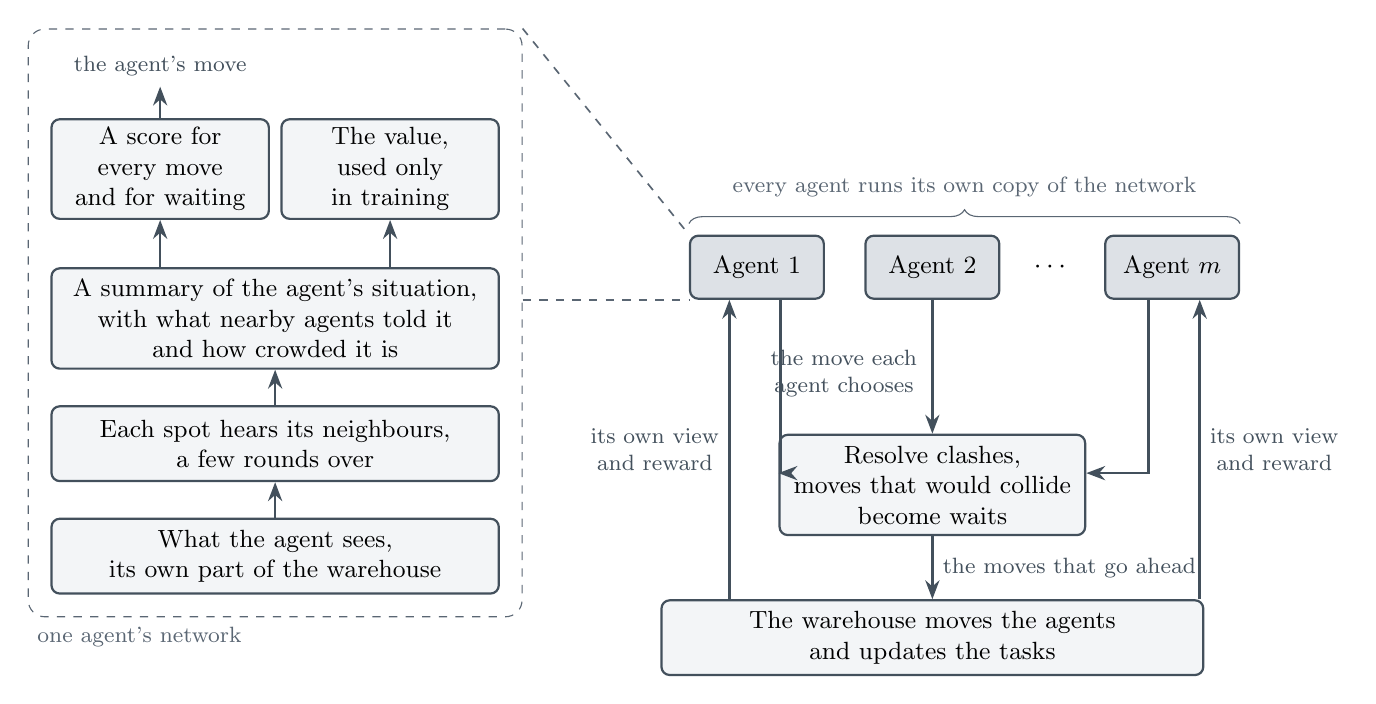
\begin{tikzpicture}
  % ---------------------------------------------------------- the network
  \node[layer] (in) {What the agent sees,\\ its own part of the warehouse};
  \node[layer, above=0.45cm of in] (mp) {Each spot hears its neighbours,\\ a few rounds over};
  \node[layer, above=0.45cm of mp] (ro) {A summary of the agent's situation,\\
    with what nearby agents told it\\ and how crowded it is};
  \node[head, above=0.6cm of ro.north west, anchor=south west] (pi)
    {A score for every move\\ and for waiting};
  \node[head, above=0.6cm of ro.north east, anchor=south east] (V)
    {The value,\\ used only\\ in training};

  \draw[flow] (in) -- (mp);
  \draw[flow] (mp) -- (ro);
  \draw[flow] (ro.north -| pi) -- (pi);
  \draw[flow] (ro.north -| V) -- (V);
  \draw[flow] (pi.north) -- ++(0,0.4) node[above, lbl] {the agent's move};

  \coordinate (nettop) at ($(pi.north)+(0,0.85)$);
  \begin{scope}[on background layer]
    \node[draw=muted, dashed, rounded corners=6pt, inner sep=8pt,
          fit=(in)(pi)(V)(nettop)] (net) {};
  \end{scope}
  \node[font=\footnotesize, text=muted, anchor=north west]
    at (net.south west) {one agent's network};

  % ---------------------------------------------------------- the loop
  \node[agent, right=2.4cm of ro.north east, anchor=west] (a1) {Agent 1};
  \node[agent, right=0.5cm of a1] (a2) {Agent 2};
  \node[right=0.3cm of a2] (dots) {$\cdots$};
  \node[agent, right=0.3cm of dots] (am) {Agent $m$};

  \draw[decorate, decoration={brace, amplitude=5pt, raise=4pt}, draw=muted]
    (a1.north west) -- (am.north east)
    node[midway, above=10pt, font=\footnotesize, text=muted]
    {every agent runs its own copy of the network};

  \node[sys, fill=shareF, text width=3.6cm, below=1.7cm of a2] (cr)
    {Resolve clashes,\\ moves that would collide\\ become waits};
  \node[sys, fill=shareF, text width=6.6cm, below=0.8cm of cr] (env)
    {The warehouse moves the agents\\ and updates the tasks};

  \draw[flow] (env.north -| a1) ++(-0.35,0) -- ($(a1.south)+(-0.35,0)$)
    node[pos=0.5, left, lbl] {its own view\\ and reward};
  \draw[flow] (env.north -| am) ++(0.35,0) -- ($(am.south)+(0.35,0)$)
    node[pos=0.5, right, lbl] {its own view\\ and reward};

  \draw[flow] ($(a1.south)+(0.3,0)$) |- ($(cr.west)+(0,0.15)$);
  \draw[flow] (a2.south) -- (cr.north);
  \draw[flow] ($(am.south)+(-0.3,0)$) |- ($(cr.east)+(0,0.15)$);
  \node[lbl, above left=0.35cm and 2pt of cr.north] {the move each\\ agent chooses};
  \draw[flow] (cr) -- node[right, lbl] {the moves that go ahead} (env);

  % zoom lines from the network to agent 1
  \draw[muted, dashed, line width=0.6pt] (net.north east) -- (a1.north west);
  \draw[muted, dashed, line width=0.6pt] (a1.south west -| net.east) -- (a1.south west);
\end{tikzpicture}
\end{document}
